\section{Agente de micro-ROS}
\label{section:microrosagent}

El agente de micro-ROS es un componente fundamental del framework de micro-ROS. Sirve de intermediario entre los nodos de micro-ROS en el microcontrolador y los nodos de ROS2 en el sistema del ordenador. En este caso particular, se ejecutará micro-ROS en Linux a través de la WSL. Para lograr esto, utiliza la implementación eProsima Micro XRCE-DDS del protocolo DDS para conectar las funcionalidades de micro-ROS con las funcionalidades más extensas de ROS2 \cite{MicroXRCE-DDS2023}.

Existen varias formas de ejecutar el agente de micro-ROS, dos de las cuales se detallan a continuación:

\subsection{Usando un repositorio de micro-ROS}

Una opción para ejecutar el agente de micro-ROS es a través de un repositorio de micro-ROS. La instalación de dicho repositorio se realiza de manera sencilla siguiendo los primeros pasos del tutorial oficial de micro-ROS\footnote{First micro-ROS Application on Linux: \url{https://micro.ros.org/docs/tutorials/core/first_application_linux/}}.

Para ejecutar el agente, se utiliza la utilidad \textit{micro\_ros\_agent} incluida en el repositorio:

\begin{verbatim}
ros2 run micro_ros_agent micro_ros_agent [transport] [options]
\end{verbatim}

El parámetro [transport] especifica el tipo de transporte utilizado para la comunicación (por ejemplo, udp, serial, etc.). Los [options] son argumentos adicionales específicos del tipo de transporte seleccionado.

Por ejemplo, el siguiente comando utiliza una comunicación serial a través del dispositivo \texttt{/dev/ttyUSB0}:

\begin{verbatim}
ros2 run micro_ros_agent micro_ros_agent serial /dev/ttyUSB0
\end{verbatim}

Para ejecutar cualquier comando de ROS2, es necesario inicializar previamente el entorno de ROS2.

\subsection{Uso de Docker para ejecutar el agente de micro-ROS}

Alternativamente, es posible utilizar Docker para ejecutar el agente de micro-ROS. Inicialmente, se debe iniciar el daemon de Docker con el siguiente comando:

\begin{verbatim}
sudo dockerd
\end{verbatim}

Posteriormente, hay que ejecutar el agente de micro-ROS utilizando el siguiente comando:

\begin{verbatim}
sudo docker run -it --rm -v /dev:/dev --privileged --net=host
microros/micro-ros-agent:humble serial --dev /dev/ttyUSB0 -v6
\end{verbatim}

Este comando ejecuta el agente de micro-ROS dentro de un contenedor Docker, otorgándole acceso a los dispositivos del sistema anfitrión y configurando la red del contenedor para utilizar la red del sistema anfitrión. En este caso, se está utilizando el agente de micro-ROS para la versión ``humble'' de ROS, utilizando una conexión serial a través del dispositivo \texttt{/dev/ttyUSB0}.

\begin{figure}[ht]
   \centering
    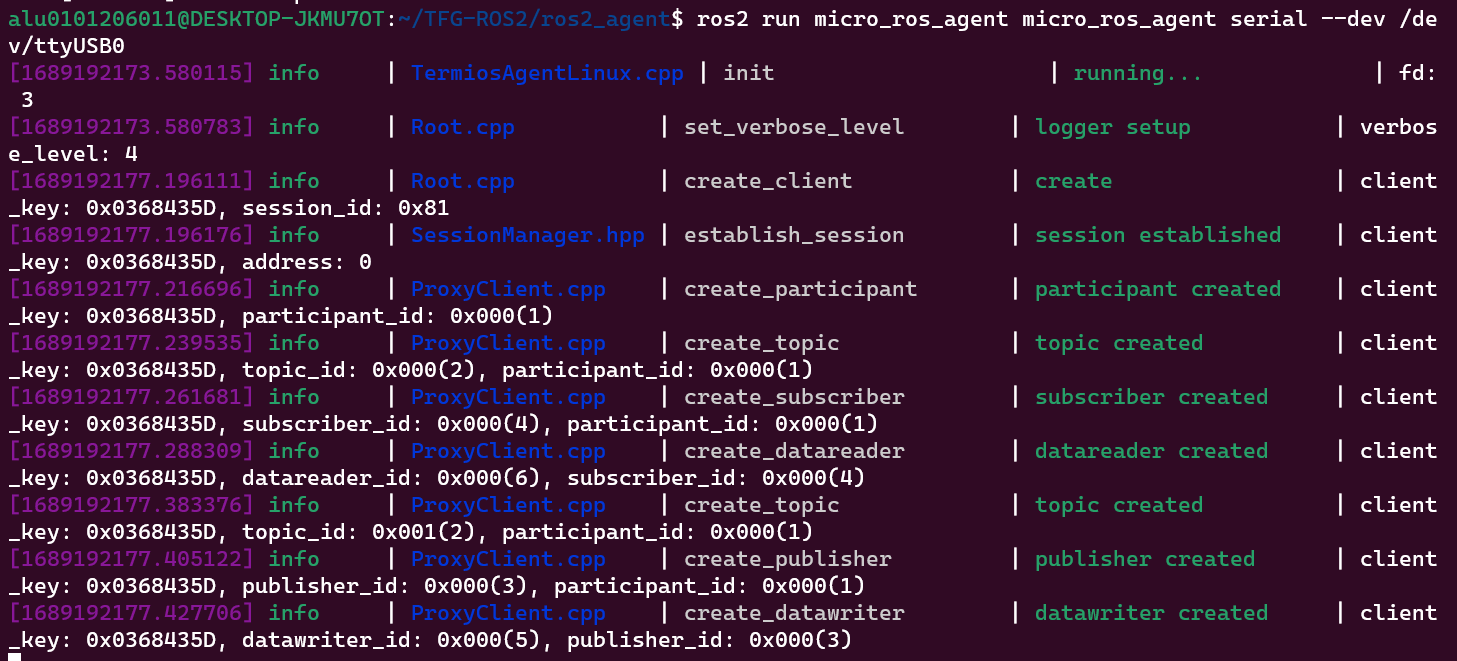
\includegraphics[width=1\linewidth]{figures/ros-agent.png}
   \caption{Ejecución del agente de micro-ROS}
   \label{figure:microrosagent}
\end{figure}


\subsection{Consideraciones adicionales}

El funcionamiento de micro-ROS depende de la ejecución de un programa agente que expone los nodos de ROS2 creados en un microcontrolador de modo que sean visibles para toda la red accesible por ROS2. El agente micro-ROS puede comunicarse con el dispositivo micro-ROS de dos formas: por comunicación serial o mediante el protocolo UDP. En el primer caso, la comunicación entre el programa micro-ROS en el dispositivo y el agente no es problemática porque el programa conecta directamente con el agente con el sistema serial. Sin embargo, si se usa UDP por ejemplo en una red wifi, hay que proporcionar al programa micro-ROS, la dirección y el puerto del agente dentro de esa red. El problema radica en que el subsistema windows de linux no es accesible directamente utilizando la IP asignada por Windows a la interfaz de red virtual creada para WSL. Se puede crear una pasarela para comunicarse con una aplicación en WSL mediante la herramienta netfs, pero bajo el protocolo TCP, y no funciona en la actualidad para el protocolo UDP. La solución para no depender de un ordenador adicional bajo linux, pasaría por utilizar una máquina virtual Virtual box en Windows para ejecutar el agente, ya que este sistema sí admite la creación de un puente con el interfaz de red wifi.
